%preamble
\documentclass[12pt,a4paper]{article}

%inputs for firstpage
\def \CourseName {گزارش فاز دوم}
\def \Instructor {دکتر مسلم حبیبی}
\def \Semester {نیم‌سال دوم\\سال تحصیلی 99-00}


%packages
\usepackage[]{algorithm2e}
\usepackage{cite}
\usepackage{calc}
\usepackage{fancyhdr}
\usepackage{lipsum}
\usepackage{color}
\usepackage{ragged2e}
\usepackage[inline]{enumitem}
\usepackage[dvipsnames]{xcolor}
\usepackage{graphicx}
\usepackage{wrapfig}
\usepackage{float}
\usepackage[skip=12pt,indent=2em]{parskip}
\usepackage{setspace}
\usepackage{textcomp}
\usepackage{etoolbox}
\usepackage{xpatch}
\usepackage{tabu}
\usepackage{hyperref}


%for persian fonts
\usepackage{xepersian}
\defpersianfont\bnazanin{BNazanin}
\settextfont{BNazanin}

\title{
	\center
	
\includegraphics[width=5cm, height=5cm]{images/shariflogo.jpg} \\
	دانشکده مهندسی صنایع \\
	دانشگاه صنعتی شریف \\
	\CourseName
}
\author{
	\\
	\\
	\textbf{استاد درس:}
	\\
	\Instructor \\[35pt]
	\\
	\textbf{نام اعضای گروه:}
	\\مهدی محسنی 
	\\محراب کشاورز گیلده 
	\\احسان چشمی
	\\[45pt]
}
\date{{\small\Semester}}


%body
\begin{document}

\maketitle
\pagebreak
\tableofcontents
\pagebreak
\normalsize	

\section{نمودار موردکاربرد} \label{section.useCase}


\section{نمودارهای فعالیت} \label{section.activity}


\subsection{فرایند ثبت نام} \label{section.activity.register}


\subsection{فرایند خرید} \label{section.activity.buy}


\subsection{فرایند مرجوعی} \label{section.activity.return}


\section{نمودارهای توالی} \label{section.sequence}


\subsection{فرایند ثبت نام} \label{section.sequence.register}


\subsection{فرایند خرید} \label{section.sequence.buy}


\subsection{فرایند مرجوعی} \label{section.sequence.return}



\pagebreak

\section{گزارش نحوه انجام پروژه} \label{section.report}

\subsection{جلسه \lr{post mortem}} \label{section.report.postMortem}

\pagebreak

\subsection{\lr{Task board and Burndown Chart}} \label{section.report.taskBoard}
		\begin{figure}[h!]
		\begin{center}
			\includegraphics[width=9cm]{images/screenshot_1.png}	
		\end{center}
		\caption{ابتدای اسپرینت-بخش اول}
	\end{figure}
	
	\begin{figure}[h!]
		\begin{center}
			\includegraphics[width=9cm]{images/screenshot_2.png}
		\end{center}
		\caption{ابتدای اسپرینت-بخش دوم}
	\end{figure}
		\begin{figure}[h!]
		\begin{center}
			\includegraphics[width=9cm]{images/screenshot_3.png}	
		\end{center}
		\caption{ابتدای اسپرینت-بخش سوم}
	\end{figure}
	
	\begin{figure}[h!]
		\begin{center}
			\includegraphics[width=9cm]{images/screenshot_4.png}
		\end{center}
		\caption{انتهای اسپرینت-بخش اول}
	\end{figure}
		\begin{figure}[h!]
		\begin{center}
			\includegraphics[width=9cm]{images/screenshot_5.png}	
		\end{center}
		\caption{انتهای اسپرینت-بخش دوم}
	\end{figure}
	
	\begin{figure}[h!]
		\begin{center}
			\includegraphics[width=9cm]{images/screenshot_6.png}
		\end{center}
		\caption{انتهای اسپرینت-بخش سوم}
	\end{figure}

\pagebreak


\begin{figure}[h!]
	\begin{center}
		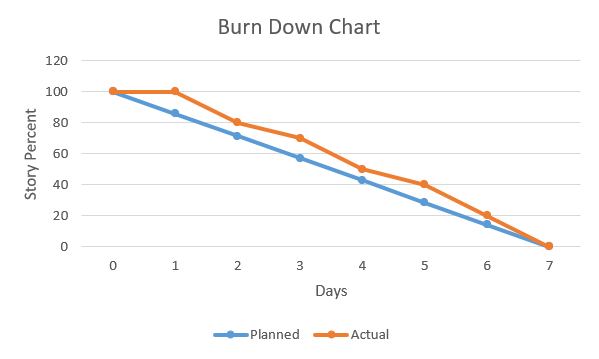
\includegraphics[width=14cm]{images/Burn Down Chart.png}
		
	\end{center}
	\caption{\lr{Burn Down Chart}}
\end{figure}




\end{document}